% -----------------------------------------------------------
% Template of theses at IPA and University of Stuttgart
% The template has been generated using Texmaker and MikTex.
% Both programs are available on Windows and
% Ubuntu (16.04 onwards).
% -----------------------------------------------------------
% Some commands need latex to be executed twice, namely:
% - Bibliography
% - Acronyms
% Therefore, configure Texmaker as follows (Options->
% Configure Texmaker->Quick Build):
% PdfLaTex + Bib(la)tex + PdfLaTex (x2) + View Pdf
% -----------------------------------------------------------
% Zotero can be used to manage the bibliography and export it
% afterwards to the BibLaTex format. Hereby, the bibliography
% is stored to resources/bibliography.bib.
% -----------------------------------------------------------
% The template offers two customizable variables in main.tex
% to set an author and a headline for the acronyms page.
% The titlepage can be modified in titlepage.tex.
% Furthermore, a sample page is included in introduction.tex
% that presents some commands and conventions.




\documentclass[12pt, a4paper, twoside]{report}

% force List of Algorithms to have grouped entries as LoF/LoT as well
\usepackage{etoolbox}
\makeatletter
\patchcmd{\@chapter}% <cmd>
  {\chaptermark{#1}}% <search>
  {\chaptermark{#1}%
   \addtocontents{loa}{\protect\addvspace{10\p@}}}% replace
  {}{}% <success><failure>
\makeatother

\usepackage{graphicx} % include images
\usepackage{subcaption}  % allows subfigures
\usepackage[export]{adjustbox}  % allows overwriting default placement of images (left)
\usepackage[footskip=1.5cm]{geometry}  % change page margins for titlepage
\usepackage{titlesec}  % change chapter layout, change title spacing (before/after)
\usepackage{titleps}  % change page numering
\usepackage{float}  % force positioning
\usepackage{hyperref}  % clickable links for table of contents
\usepackage[english]{babel}  % English hyphenation style
% \usepackage[ngerman]{babel} % German version
\usepackage{microtype}  % improves full justification
\usepackage{fancyhdr}  % further customize page layout (decorative lines, etc)
\usepackage{setspace}  % control line spacing
\usepackage[nottoc]{tocbibind}  % list LoF and LoT in table of contents
\usepackage{acro}  % package for listing acronyms
\usepackage{tabu,longtable}  % redefine table format for acronyms
\usepackage{amssymb}  % more symbols
\usepackage{amsmath}  % better math formulas
\usepackage{tabularx} % auto line break for tables
\usepackage{booktabs} % nicer tables
\usepackage{algorithm}  % algorithm environment for pseudo code
\usepackage{algpseudocode}  % write pseudo code
\usepackage[labelsep=period]{caption}  % period instead of colon as delimiter in figure/table, and multi page subfigures
\usepackage[backend=bibtex, citestyle=ieee, style=numeric, maxbibnames=99]{biblatex}
\usepackage[T1]{fontenc}  % support special characters of authors in bib
\usepackage[utf8]{inputenc}
\usepackage{lmodern}  % scalable fonts, needed with fontenc, changes font to latin modern
\usepackage{relsize}  % for hack concerning underscore length
\usepackage{appendix}  % appendix
\bibliography{resources/bibliography.bib}


% user definable settings
\newcommand{\acronymtitle}{List of Acronyms}  % chapter header for acronyms page
\newcommand{\authorname}{Max Sample}  % author of thesis
% end settings


% change default chapter layout
\titleformat{\chapter}%
  {\normalfont\bfseries\huge\setstretch{1.0}}{\thechapter.}{12pt}{}
\titlespacing*{\chapter}{0pt}{0pt}{20pt}

% define header and footer
\pagestyle{fancy}
\fancyhf{} % clear all fields
\fancyhead[LE,RO]{\slshape\nouppercase\leftmark}
\fancyhead[CO,CE]{\slshape{\authorname}}
\fancyfoot[LE,RO]{\slshape\thepage}
\renewcommand{\headrulewidth}{0.4pt}  % fancy line in header
\renewcommand{\footrulewidth}{0.4pt}  % fancy line in footer
\renewcommand{\chaptermark}[1]{\markboth{\thechapter.\space#1}{}}  % remove Chapter tag from header

% overwrite chapter pages which fall back to plain style
\fancypagestyle{plain}{%
	\fancyhf{}
	\fancyhead[LE,RO]{\slshape\nouppercase\leftmark}
	\fancyhead[CO,CE]{\slshape{\authorname}}
	\fancyfoot[LE,RO]{\slshape\thepage}
	\renewcommand{\headrulewidth}{0.4pt}
	\renewcommand{\footrulewidth}{0.4pt}
}

% invert twoside layout
\let\tmp\oddsidemargin
\let\oddsidemargin\evensidemargin
\let\evensidemargin\tmp
\reversemarginpar

% set line spacing to 1.5
\setstretch{1.5}

% remove default left indent for LoT, LoF and LoA
% the second parameter is responsible for that and forced to 0pt
% others are kept at default values
\makeatletter
\let\old@dottedtocline\@dottedtocline
\renewcommand{\@dottedtocline}[5]{\old@dottedtocline{#1}{0pt}{#3}{#4}{#5}}
\makeatother

% reduce the hspace before and after equations
\AtBeginDocument{
\setlength{\abovedisplayskip}{4pt}
\setlength{\abovedisplayshortskip}{2pt}
\setlength{\belowdisplayskip}{6pt}
\setlength{\belowdisplayshortskip}{4pt}
}

% add chapter number to algorithm counting
% further, reset algorithm counter for each new chapter
\makeatletter 
\renewcommand\thealgorithm{\thechapter.\arabic{algorithm}} 
\@addtoreset{algorithm}{chapter} 
\makeatother

\setlength{\parskip}{0pt} % avoid latex to put space between paragraphs

\renewcommand{\_}{\textscale{.3}{\textunderscore}}  % hack for shorter underscores in lmodern font

% acronyms have to be defined in the preamble
\DeclareAcroListStyle{longtabu}{table}{
	table=longtabu,
	table-spec=@{}>{\bfseries}lX@{},  % first column bold
	before = \singlespacing\renewcommand\arraystretch{1.655}  % avoid new rows for long entries, optimized for 12pt fonts here
}

\acsetup{
	list-heading=chapter*,
	list-style=longtabu,
	list-name={\acronymtitle},
	extra-style=paren,
	hyperref=true
}

% List of acronmys
\DeclareAcronym{ipa}{
  short = IPA,
  long  = Institute for Manufacturing Engineering and Automation,
  list = Institut f\"ur Produktionstechnik und Automatisierung\newline,
  extra = English: Institute for Manufacturing Engineering and Automation\vspace*{6pt}
}

\DeclareAcronym{cnn}{
  short = CNN,
  long  = convolutional neural network,
  list  = Convolutional Neural Network
}

\DeclareAcronym{cob4}{
  short = COB 4,
  long  = Care-O-bot 4,
  extra = Service Robot
}


\begin{document}

	\begin{titlepage}

	\newgeometry{top=3cm, hmarginratio=1:1}
	
	\begin{figure}
		\begin{subfigure}{0.5\textwidth}
			
\includegraphics[width=1.1\linewidth, left]{resources/logos/university_stuttgart_logo}
		\end{subfigure}
		\begin{subfigure}{0.5\textwidth}
			
\includegraphics[width=0.8\linewidth, right]{resources/logos/ipa_logo}
		\end{subfigure}
	\end{figure}
	
	\begin{center}
	
		\vspace*{0.5cm}
		
		\huge
		\textbf{Title of my Thesis}
		
		\vspace{0.25cm}
		
		\Large
		Subtitle of my Thesis
		
		\vspace{1cm}
		
		\textbf{\authorname}
		
		\vspace{1cm}
		
		A thesis presented for the degree of\\
		Master of Science
		
		\vfill
		
		\begingroup
			\setstretch{1.2}
			\begin{tabular}{r l l}
				\textbf{Supervisors}: & \ & <Enter Supervisor>\\
									& \  & <Enter University Superisor>\\[2mm]
				\textbf{Examiner}: & \  & <Enter Examiner>
			\end{tabular}
		
			\vspace{1cm}
		
			\large
			\begin{tabular}{r l l}
				Department Name: & \ & Fraunhofer Institute for\\
				& \ & Manufacturing Engineering and Automation\\[1mm]
				University Name: & \ & University of Stuttgart\\[1mm]
				Date: & \ & December 9th, 2019\\
			\end{tabular}
		\endgroup	
		
	\end{center}
	
\end{titlepage}
	\restoregeometry
	\newpage\null\thispagestyle{empty}\newpage  % add blank page
	\pagenumbering{roman}
	\addtocounter{page}{2}  % count pages from title page on
	
	\chapter*{Declaration of Authorship}
\label{sec:declaration}
\markboth{Declaration of Authorship}{}  % add something of work to page header
I hereby certify that the present thesis has entirely been developed and written by myself. Passages, ideas and materials from other sources have clearly been marked with a citation and an indication of the source. Furthermore, this thesis has never been submitted in the same or substantially similar version to any other authority to achieve an academic grading.

\hspace{1cm}

\begin{flushright}
Stuttgart, Dec 1st, 2019 \hphantom{\authorname}\hspace{1.5cm}

\begin{tabular}{r}
	\hline
	\hspace{1cm}\authorname
\end{tabular}
\end{flushright}

	\newpage\null\thispagestyle{empty}\newpage  % add blank page

	\chapter*{Abstract}
\label{sec:abstract}
\markboth{Abstract}{}  % add title of work to page header
To be filled.

	\newpage\null\thispagestyle{empty}\newpage  % add blank page
	
	\tableofcontents
	\clearpage

	\listoffigures
	\listoftables
	\listofalgorithms
	\addcontentsline{toc}{chapter}{List of Algorithms}

	\clearpage % end page so that "List of Algorithms" header does not carry over
	\markboth{\acronymtitle}{}  % add Acronyms to page header
	\acuseall  % acro is still buggy and does not show all acronyms sometimes
	\printacronyms
	\addcontentsline{toc}{chapter}{\acronymtitle}
	\clearpage % end list of acronyms
	\acresetall  % reset acronyms as some might be listed in the list of figures/tables so that long forms will be printed once again in text

	% add blank page if the page after acronyms is even so that the introduction starts on an uneven page
	\makeatletter\ifodd\c@page\else
		\newpage\null\thispagestyle{empty}\newpage
	\fi\makeatother
	\pagenumbering{arabic}  % starts at 1, which is uneven (even when this should actually be an even page number) which can break the layout style
	
	\chapter{Introduction}
\label{chp:introduction}
\Acp{cnn} are great \cite{goodfellow_deep_2016} because a \ac{cnn} is good at classifying images.

% An empty line between text starts a new paragraph
A depiction of the gripper of the \ac{cob4} used at \ac{ipa} is given in Figure~\ref{fig:Grippers}. % References (figures, tables, equations, algorithms, chapters, etc... ) always with capital letter.

\par\bigskip  % some further space, can also be used between subfigures for more vertical space
%\par\medskip
%\par\smallskip

\begin{figure}[htbp]
	\centering
	\begin{subfigure}{0.49\textwidth}
		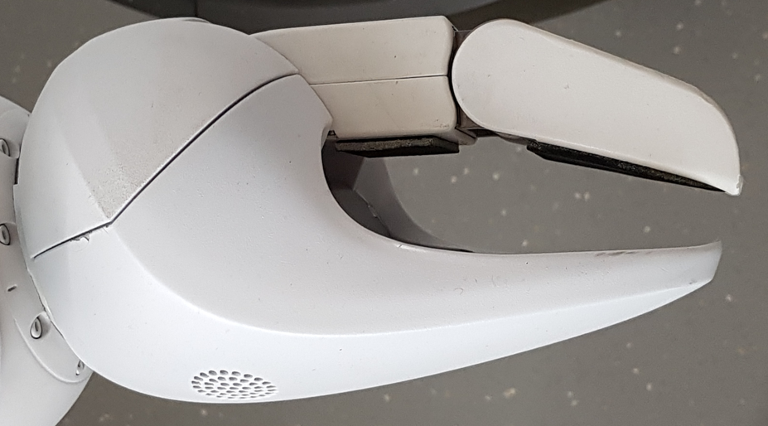
\includegraphics[height=0.15\textheight, center]{resources/figures/introduction/cob4_gripper}
		\caption{Real-World}
	\end{subfigure}
	\begin{subfigure}{0.49\textwidth}
		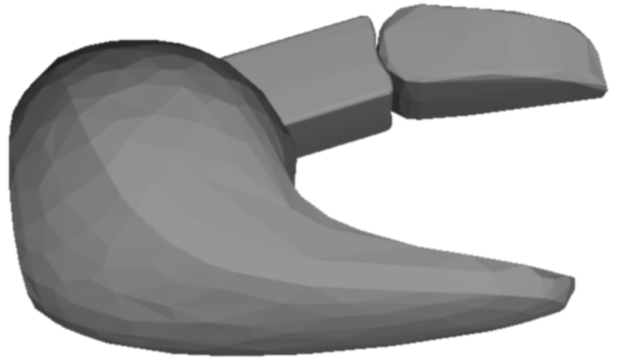
\includegraphics[height=0.15\textheight, center]{resources/figures/introduction/cob4_gripper_sim}
		\caption{Simulation}
	\end{subfigure}
	\caption[Two-finger gripper of the \acs{cob4}]{Two-finger gripper of the \acs{cob4} used at \acs{ipa}}  % caption below images
	\label{fig:Grippers}
\end{figure}
% Use always the short (e.g. acs) version for acronyms in captions to avoid having the full string printed in the list of figures. Take a look at the documentation of the acro package for further information.

\noindent Some hyperparameters are explained in Table~\ref{tab:hyperparameters} below.  % \noindent suppresses the paragraph indentation

% Nice tables only have horizontal lines. Avoid vertical lines for a better appearance.
\begingroup
\renewcommand\arraystretch{1.3}  % more space between rows (also affects equations, therefore use a local group)
\begin{table}[b!]  % force on bottom
\centering
\caption{Hyperparameters}  % caption above tables
\label{tab:hyperparameters}
\begin{tabularx}{\linewidth}{lX}
	\toprule
	\textbf{Parameter} & \textbf{Description}\\
	\midrule
Learning Rate & This is the most important hyperparameter to tune. It defines the stepsize to take in negative gradient direction to reduce the overall error of the neural network.\\
Batch Size & This specifies the amount of samples processed in one update of the neural network.\\
	\bottomrule
\end{tabularx}
\end{table}
\endgroup


	
	\chapter{State of the Art}
\label{chp:stateoftheart}
To be filled.

	
	\chapter{Fundamentals}
\label{chp:fundamentals}
To be filled.


	\chapter{Conception}
\label{chp:conception}
To be filled.

	
	\chapter{Implementation}
\label{chp:implementation}
To be filled.

	
	\chapter{Experiments}
\label{chp:experiments}
To be filled.

	
	\chapter{Conclusion}
\label{chp:conclusion}
To be filled.

	
	\begin{appendices}
	\chapter{Title of Appendix 1}
\label{app:appendix1}
To be filled.

\chapter{Title of Appendix 2}
\label{app:appendix2}
To be filled.
	\end{appendices}
	
	\printbibliography[heading=bibintoc]
  
\end{document}
